\subsection{Problemas}
--------------------------------------------------------
\\

\np

\begin{enumerate}[label=\alph*)]
    \item Un disco cargado con una densidad de carga eléctrica uniforme $\sigma$ se hace girar. Si gira a una velocidad angular $\omega$, determine la densidad de corriente superficial $\Vec{K}$.
    \item Una esfera sólida centrada en el origen de coordenadas y uniformemente cargada, de radio $R$ y de carga total $Q$, gira con una velocidad angular constante $\omega$ alrededor del eje $z$ ($\Vec{\omega}=\omega\hat{z}$). Determine la densidad de corriente volumétrica $\Vec{J}$ en cualquier punto $(r, \theta, \phi)$ dentro de la esfera.
\end{enumerate}

\bigbreak

\np

\begin{enumerate}[label=\alph*)]
    \item Suponga que se construye un cono truncado, como se muestra en la figura, usando un material de resistividad $\eta$. Determine la resistencia entre las caras $A$ y $B$.
    \item  Suponga que ahora se tiene un trozo de cilindro, como se muestra en la figura, de un material de conductividad $g$. Determine la resistencia entre las caras $A$ y $B$. Luego entre las caras $C$ y $D$, y finalmente entre las caras $E$ y $F$.
\end{enumerate}

\begin{figure}[H]
    \centering
    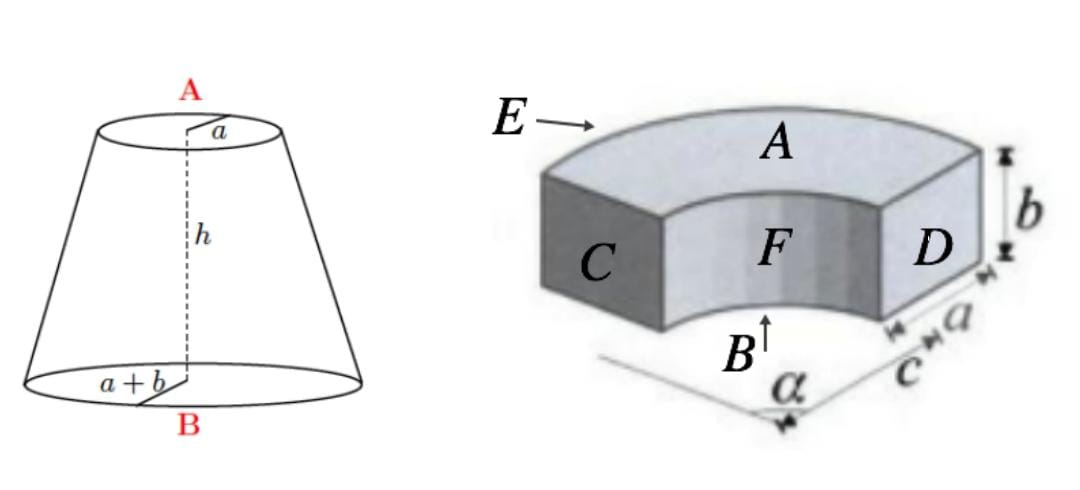
\includegraphics[width=0.7\textwidth]{Corriente/Imagen1.jpeg}
\end{figure}

\bigbreak

\np

Una corriente estacionaria fluye por un cilindro de largo $l$ y radio $a\ll l$ hecho de un material semiconductor que obedece la ley de Ohm y cuya conductividad viene dada por $g(x) = g_oe^{x/l}$, donde $x$ es la distancia a lo largo del eje del cilindro, mientras que $g_o$ es una constante conocida. Ambos extremos están conectados a cilindros conductores perfectos del mismo radio que el semiconductor. Suponga además que $V(0) = V_0$ y $V(l) = 0$, y que la densidad de corriente es uniforme.

\begin{enumerate}[label=\alph*)]
    \item Calcule la resistencia del semiconductor y la corriente que lo atraviesa.
    \item Encuentre el potencial como función de la posición $V (x)$.
    \item Determine las cargas libres presentes en el sistema.
    \item Durante el régimen estacionario, ¿existe variación de energía electrostática almacenada en el sistema?. ¿Existe energía disipada a lo largo del tiempo? Si su respuesta es positiva, ¿a dónde va esta energía? ¿De dónde viene esta energía?
    \item Si la fuente externa se desconectara, explique cualitativamente qué pasaría con las cargas libres del sistema.
    \item Durante el periodo transitorio, determine cuál sería la variación de energía electrostática almacenada en el sistema. ¿Cuánta energía se disiparía por efecto Joule durante este periodo?
\end{enumerate}

\begin{figure}[H]
    \centering
    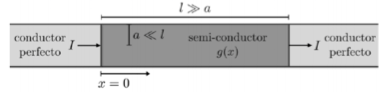
\includegraphics[width=0.7\textwidth]{Corriente/cilindro_P_9_3.png}
\end{figure}

\bigbreak
\np

Entre dos placas planas y paralelas separadas una distancia $a+b$ se coloca una capa de espesor $a$ de un medio de permitividad $\epsilon$ y conductividad $g$. El resto del espacio lo ocupa una capa de espesor $b$ vacía. En el instante $t = 0$ se conecta una diferencia de potencial $V_0$.

\begin{enumerate}[label=\alph*)]
    \item ¿Cuánto valen $\Vec{E}$, $\Vec{D}$ y $\Vec{J}$ inmediatamente después de conectar el potencial?
    \item ¿Cuánto valen un tiempo largo después de que se haya establecido? (estado estacionario)
    \item ¿Cuánto valen en cualquier instante?
    \item Determine las cargas presentes en el sistema (libres y polarización) en función del tiempo.
    \item  ¿Cómo varía, durante el periodo transitorio, la energía almacenada en el sistema? ¿Cuánta energía se disipa durante este periodo? ¿De dónde procede esta energía?
\end{enumerate}

\begin{figure}[H]
    \centering
    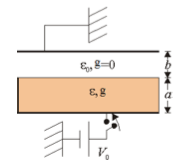
\includegraphics[width=0.3\textwidth]{Corriente/PlacaP_9_4.png}
\end{figure}

\bigbreak
\np

Se tienen dos cascarones esféricos conductores perfectos de radios $a$ y $b$. El conductor interno se carga con $Q_0$ mientras que el conductor externo se mantiene conectado a tierra. Considerando que la mitad del espacio entre ambos conductores está lleno con un material de constante dieléctrica $\epsilon$ y conductividad $g$, determine:

\begin{enumerate}[label=\alph*)]
    \item La evolución en el tiempo de la carga en la esfera interior, y de los campos $\Vec{E}$ , $\Vec{J}$ y $\Vec{D}$ en la zona entre las esferas.
    \item La intensidad de corriente que fluye por el material conductor.
    \item  La energía total disipada por el medio material. ¿Cómo se relaciona con la variación de energía electrostática del sistema?
\end{enumerate}

\bimage[0.3\textwidth]{Corriente/P_9_5.png}

\bigbreak
\np

Considere un condensador cilíndrico de radios interior $a$ y exterior $b$ y largo $L$, el cual posee al interior de él tres medios conductores de conductividad $g_1$, $g_2$ y $g_3$ y permitividad $\epsilon_o$, los cuales ocupan el mismo volumen en el condensador. El casquete interior se mantiene a un potencial $V_0$ gracias a una batería y el casquete exterior se encuentra conectado a tierra.

\begin{enumerate}[label=\alph*)]
    \item Si el condensador ha alcanzado el régimen estacionario, determine $\Vec{J}$, $\Vec{E}$, la resistencia y la corriente del sistema.
    \item Considere que ha pasado un tiempo muy largo y se desconecta la batería. Determine la corriente del sistema en función del tiempo.
    \item  ¿Cómo varía, durante el periodo transitorio, la energía almacenada en el sistema? ¿Cuánta energía se disipa durante este periodo?
\end{enumerate}

\bimage[0.35\textwidth]{Corriente/P_9_6.png}

\np

El espacio entre dos placas conductoras se rellena con dos materiales conductores, de conductividades $g_1$ ($0 < x < a$) y $g_2$ ($a < x < a + b$), y permitividad $\epsilon_o$. En $t = 0$, el material de conductividad $g_1$ se carga con una densidad volumétrica uniforme $\rho_o$, y en el mismo instante se establece una diferencia de potencial igual a $V_0$ entre las placas, mediante una batería externa, donde la superficie superior ($x = a + b$) se conecta a tierra y la superficie inferior $(x = 0)$ se conecta a un potencial $V_0$.

\begin{enumerate}[label=\alph*)]
    \item Determine los campos $\Vec{E}$ y $\Vec{J}$, y todas las cargas libres presentes en el sistema, inmediatamente después de conectar la batería.
    \item Determine los campos $\Vec{E}$ y $\Vec{J}$, y todas las cargas libres presentes en el sistema, cuando ha trascurrido un tiempo muy largo, es decir, en el estado estacionario.
    \item En el régimen estacionario, ¿existe variación de energía electrostática almacenada en el sistema?
    \item En el régimen estacionario, ¿existe energía disipada a lo largo del tiempo? Si su respuesta es positiva, ¿a dónde va esta energía? ¿De dónde viene esta energía?
\end{enumerate}

\bimage[0.5\textwidth]{Corriente/P_9_7.png}

\newpage